\section{Iteration loop}\label{iteration-loop}

In section \ref{mandelbrot-set} it was mentioned that fractals are calculated
by repeating a formula \emph{iterating} in an iteration loop. 
The integer \emph{"i"} is used to represent the \emph{iteration count} number.

The iteration count starts with i = 0, then at the end of each iteration the
count number is increased by 1, and the next iteration of the formula commences 
(e.g. iteration count  0, 1, 2, 3, ...). The iterating continues until \emph{termination conditions} are met, 
which is either when the iteration count i =  \emph{maxiter} or when the \emph({bailout}) condition is achieved. 

This section explains the calculations within the iteration loop.

A fractal formula is built from mathematical equations. 
These equations can be modifications of the Mandelbrot Set equation (e.g Mandelbulb) and also other mathematical equations.

The equations are made from mathematical operators ($+, -, *, /$) 
and can include mathematical functions (e.g. $\sin, \cos, \tan, \exp, \log, sqrt, pow, fabs$) 
and also mathematical conditions (e.g. if x > y then "compute following equation(s)", if i > 4 then "compute following equation(s)").

The equations are applied to vector z or any parts of z (i.e the z.x, z.y and z.z components)

Examples:
\emph{z.x = fabs(z.x);} is using the function fabs (i.e. z.x is assigned the absoulute value of z.x)
\emph{if ( z.x - z.y < 0.0) swap(z.x, z.y);} is using the conditional function if() to determine if the values of z.x and z.y should be swapped.
\emph{( z *= 3.0)} is using the operator * to multiply the all components of vector z by 3.0.

A set of equations that have a specific function within the formula are called \emph{transforms}, e.g rotation, scale.

The general form, is a formula is constructed from one or more transforms, which are constructed from equations.

With each iteration of the formula, the point being iterated is \emph{mapped} (moved) to new coordinates as a result of the mathematical equations.  

\subsection{Single formula fractals}\label{single-formula-fractals}

The simplest 3D fractals are calculated by iterating a single fractal formula. More complex fractals are made by iterating a mix of formulas, adding extra transforms, and/or including additional conditions. 

Below there are 3 examples of fractals formulas written in C language code

\subsubsection{Mandelbulb Power 2}\index{Mandelbulb} \nopagebreak

This formula is a modified Mandelbrot Set equation, expanded to \nth{3} dimension.
A cross section at $ z_z = 0 $ looks exactly the same as Mandelbrot Set.
\nopagebreak

\begin{tabular}{l l}
	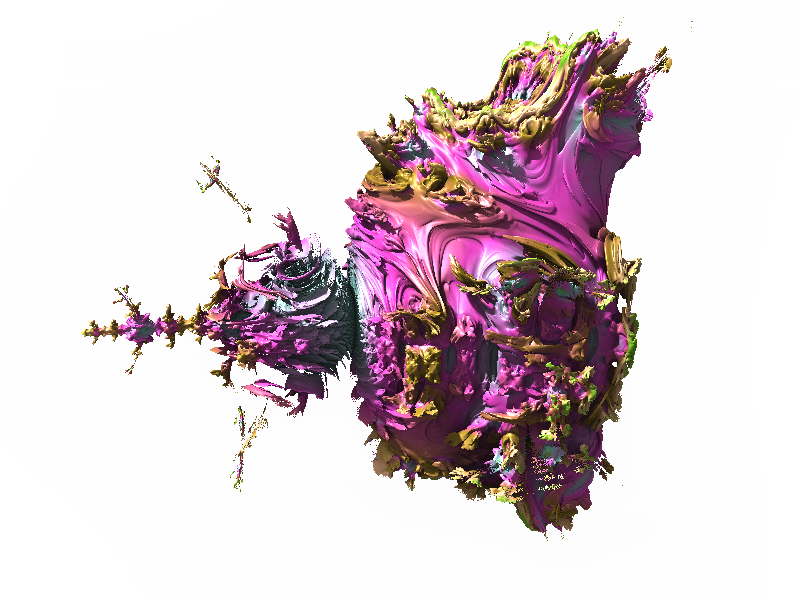
\includegraphics[width=0.3\linewidth]{img/manual/media/formula_mandelbulb_power_2}	
	& 
	\begin{minipage}[b]{0.5\linewidth}
		\lstinputlisting[caption={Formula > Mandelbulb Power 2}]{code/formula_mandelbulb_power_2.cpp}
	\end{minipage}
\end{tabular} 

\subsubsection{Menger Sponge}\index{Menger Sponge} \nopagebreak

This formula is an Iterated Function System (IFS). It contains several
transforms, some of them conditions. \nopagebreak

\begin{tabular}{l l}
	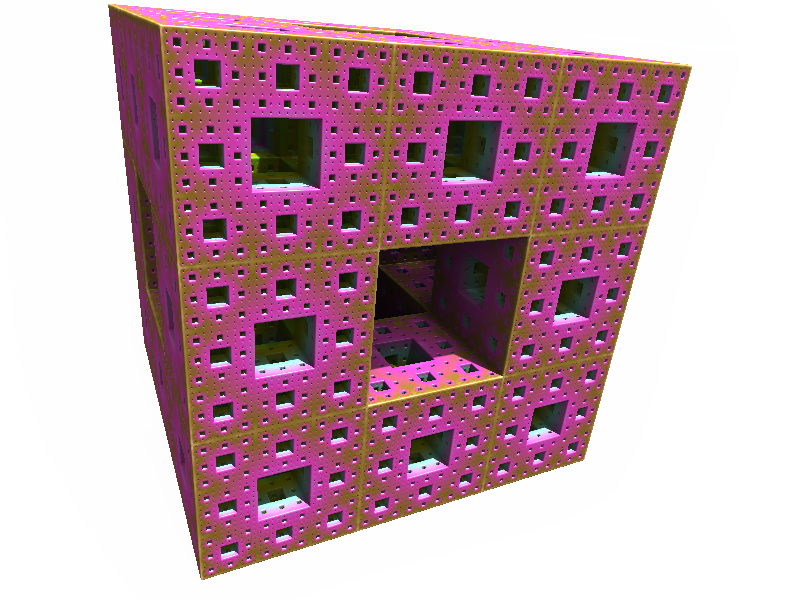
\includegraphics[width=0.3\linewidth]{img/manual/media/formula_menger_sponge.png}	
	& 
	\begin{minipage}[b]{0.5\linewidth}
		\lstinputlisting[caption={Formula > Menger Sponge}]{code/formula_menger_sponge.cpp}
	\end{minipage}
\end{tabular} 

\subsubsection{Box Fold Bulb Pow 2}

This formula is made from a set of different transforms. It is a good example of
how a fractal formula can be more complicated than the
\emph{Mandelbrot Set} formula.

First part is a ``box fold''\index{transform!box fold} transform which conditionally maps the point in x,y,z  directions. Second part is a ``spherical fold''\index{transform!spherical fold} which does conditional scaling in a radial direction.
The end of formula is the same as \emph{Mandelbulb Power 2}.

\begin{tabular}{l l}
	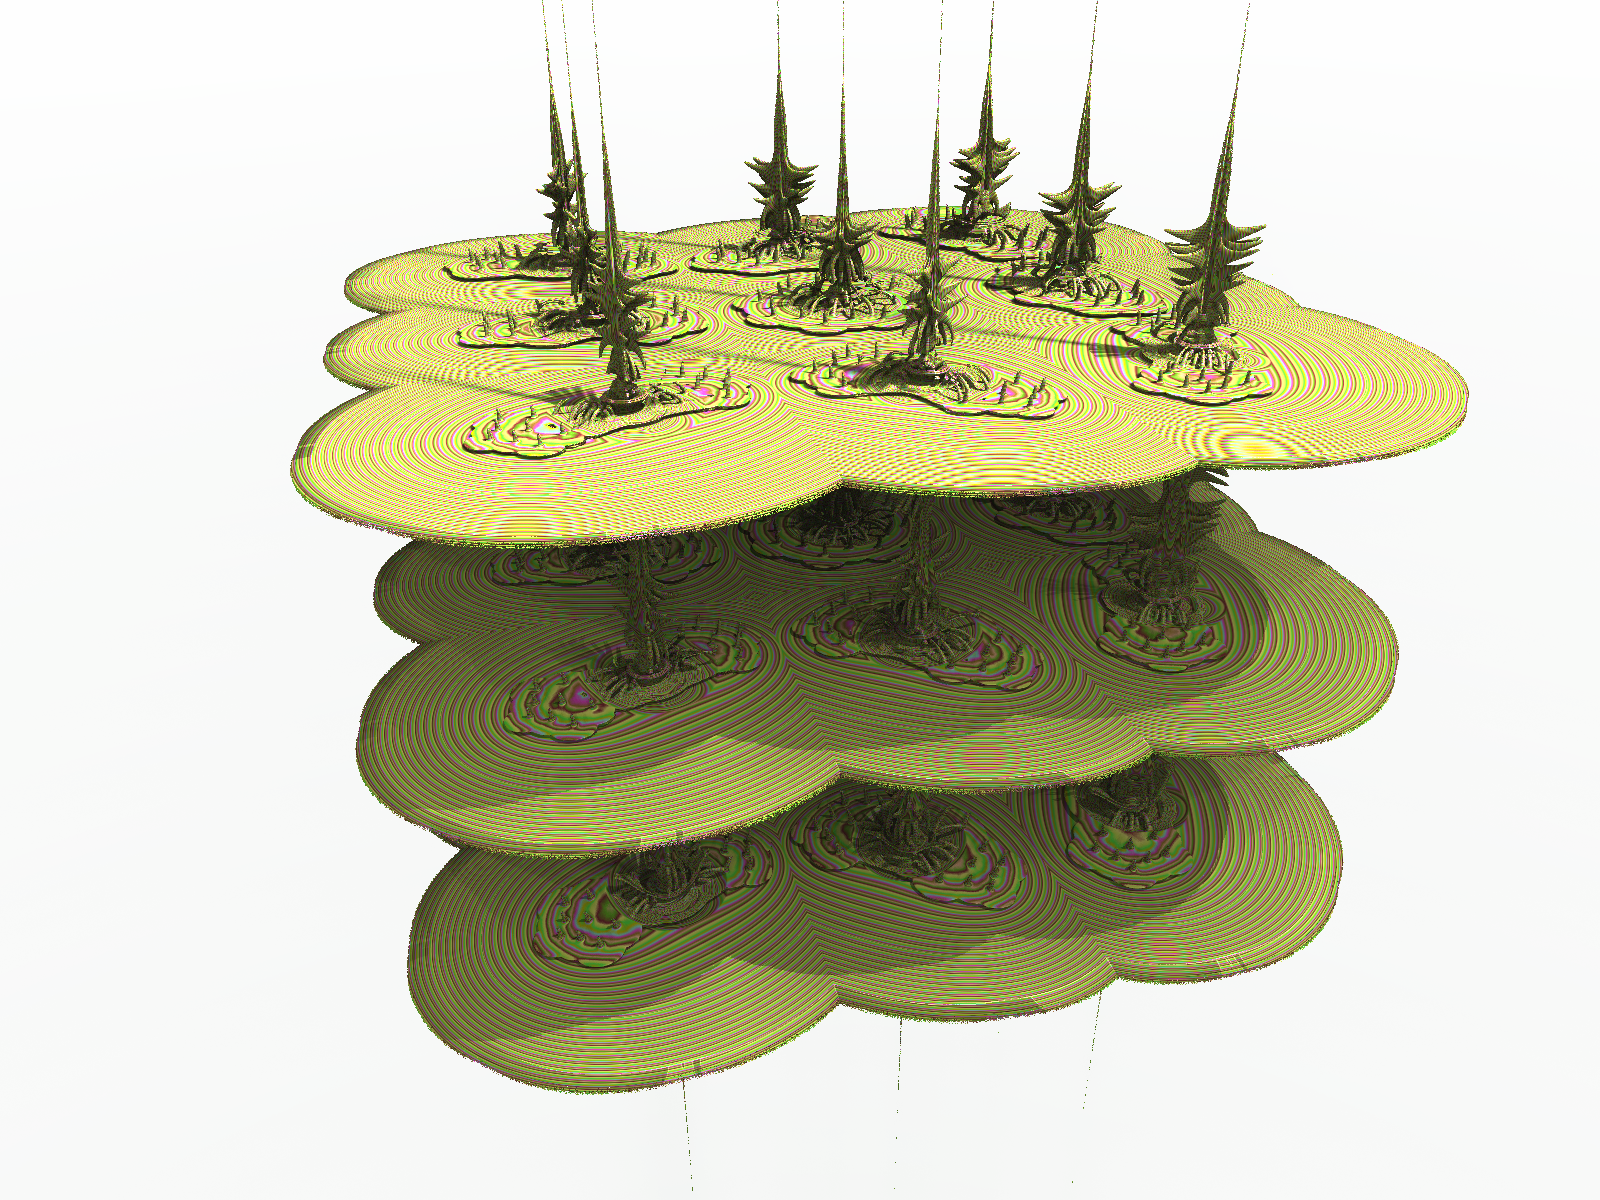
\includegraphics[width=0.3\linewidth]{img/manual/media/formula_box_fold_pwr2.png}	
	& 
	\begin{minipage}[b]{0.5\linewidth}
		\lstinputlisting[caption={Formula > Box fold Power 2}]{code/formula_box_fold_pwr2.cpp}
	\end{minipage}
\end{tabular} 

\subsubsection{Processing of single formula fractals}

Single formula fractals are simply iterated several times until termination conditions are met, as shown in figure \ref{iteration_loops}. \nolinebreak \nopagebreak


\simpleImageWithCaption75Width{img/manual/media/iteration_loops.png}
{Simple Iteration loops with one formula}
{iteration_loops}

When the calculation of the iteration loop finishes the resulting final value of \emph{z} is
used to estimate the distance to the fractal body and to calculate the color of the surface.

\subsection{Hybrid fractals}\index{fractal!hybrid}

\emph{Hybrid fractals} are constructed by using more than one formula in the iteration loop.
This way new variations of fractal shapes can be achieved. There are many different fractal formulas and transforms available in the Mandelbulber program, which allows the user to create a vast variety of hybrid shapes.

\subsubsection{Iteration loop of hybrid fractals}

In general hybrid fractals are calculated in a similar way to single formula fractals.
The calculation consists of the iteration loop, \emph{maxiter} and \emph{bailout} condition. The
difference is that when \emph{hybrid mode} is enabled, a user can create a \emph{sequence} of up to nine different fractal formulas (or transforms) inside the iteration loop. 

By default the program works in single fractal formula mode, where you can only configure the parameters of the formula tab in the first slot,
(\#1). There are two ways to enable hybrid fractals:
\begin{itemize}
	\item Click in any slot with a number higher than one. The program will ask if you want to
	enable hybrid fractals or boolean mode. Select \emph{Enable hybrid fractals}
	\item Go to \emph{Objects} / \emph{Hybrid} tab. Tick \emph{Enable hybrid fractals} checkbox.
\end{itemize}

Once hybrid fractals has been enabled, a user can select additional formulas from the dropdown menus in any of the nine formula slots,
as shown in figure \ref{fractal_tabs_with_defined_fractals_tabs_highlighted}.
In this figure \emph{Mandelbulb - Power 2} is selected in slot \#1, \emph{Menger Sponge}
in slot \#2 and \emph{Box Fold Bulb Pow 2} in slot \#3. These formulas will be
used in the next examples.

\simpleImageWithCaption75Width{img/manual/media/fractal_tabs_with_defined_fractals_tabs_highlighted.png}
{Fractal Tab - Multiple formula slots filled}
{fractal_tabs_with_defined_fractals_tabs_highlighted}

Each formula's parameters can be configured in the formula tab opened in an enabled slot.
\simpleImageWithCaption75Width{img/manual/media/fractal_tabs.png}
{Fractal Tab - Formula only in first slot}
{fractal_tabs}

The iteration count numbers determine when in the sequence each formula is calculated.

The sequence is in the order of enabled formula slots from \#1 to slot \#9, (e.g. If the sequence is calculating formulas in slots
\#1 and \#5, then the iteration loop repeats the sequence of slot \#1 calculation followed by slot
\#5 calculation.)
How the sequence will work depends on the following selections:
\begin{itemize}
	\item Which fractal formulas are selected in the formula slots
	\item How many iterations are assigned to each formula
	\item The range of iteration numbers when the formula will be used
	\item From which fractal slot the sequence will be repeated
\end{itemize}

\simpleImageWithCaption75Width{img/manual/media/iteration_loop_hybrid.png}
{Complex Iteration loop with hybrid fractal}
{iteration_loop_hybrid}

\subsubsection{One iteration for each slot}

The simplest way to create a hybrid fractal is a sequence where formulas are calculated one after another, then the sequence is repeated until termination conditions are met.

In figure \ref{iteration_loop_hybrid_sequence_1}, the sequence consists of one \emph{Mandelbulb - Power 2}, one \emph{Menger Sponge} and
one \emph{Box Fold Bulb Pow 2}. The length of the sequence is three slots, so after every third iteration the sequence repeats from the first slot. The numbers shown are the Iteration Count, starting at i = 0. The count increases by 1 after \underline{every} iteration performed in the iteration loop.

\simpleImageWithCaptionFullWidth{img/manual/media/iteration_loop_hybrid_sequence_1.png}
{Hybrid sequence - Simple sequence using three different formulas}
{iteration_loop_hybrid_sequence_1}

This sequence gives a shape combining properties of all three
formulas, see figure \ref{hybrid_sequence_example_1}.

\simpleImageWithCaptionHalfWidth{img/manual/media/hybrid_sequence_example_1.png}
{Hybrid sequence render - Simple sequence using three different formulas}
{hybrid_sequence_example_1}

Because the first iteration is (slot \#1) \emph{Mandelbulb - Power 2}, the general shape
of the fractal will be simlar in shape to the \emph{Mandelbulb - Power 2}.

\emph{Note: Generally, the first few iterations of a fractal strongly influence the final hybrid fractal shape.}

In the next iteration \emph{Menger Sponge} formula is used. A single iteration
of this formula produces the shape of figure \ref{single_iteration_of_menger_sponge}.

\simpleImageWithCaptionSmallWidth{img/manual/media/single_iteration_of_menger_sponge.png}
{Single iteration of the Menger Sponge}
{single_iteration_of_menger_sponge}

Some features of this shape are transferred to the generated shape of the hybrid fractal.

\simpleImageWithCaptionHalfWidth{img/manual/media/single_iteration_of_menger_sponge_hybrid.png}
{Hybrid with Menger Sponge features marked in red}
{single_iteration_of_menger_sponge_hybrid}

The Menger Sponge shape is distorted, because \emph{Mandelbulb - Power 2} has
already deformed the space.

The third formula \emph{Box Fold Bulb Pow 2} adds leaf-like features to the shape.

\simpleImageWithCaptionSmallWidth{img/manual/media/hybrid_sequence_example_1_leaf_shapes.png}
{Hybrid close up of leaf-like shapes produced by 'Box Fold Bulb Pow 2' formula}
{hybrid_sequence_example_1_leaf_shapes}

\subsubsection{More iterations for each slot}

With each slot a user can define how many times each fractal formula will be used in the sequence.
On each of the formula tabs there is a parameter named \emph{Iterations} which is set to 1 by default.
This is the number of iterations (repeats) of the formula performed before the loop moves on to the next formula slot in the sequence.
If this value is increased to 2 on the first and second formula slots in our example,
then the sequence of the formulas will be as shown in figure \ref{iteration_loop_hybrid_sequence_2}. \label{two-iterations-per-slot}

\simpleImageWithCaptionFullWidth{img/manual/media/iteration_loop_hybrid_sequence_2.png}
{Hybrid sequence - The first and second slots set to 2 repeat iterations}
{iteration_loop_hybrid_sequence_2}

The first and second formulas are repeated twice and the third formula only once.
The resulting fractal shape is shown in figure \ref{hybrid_sequence_example_2}:

\simpleImageWithCaptionHalfWidth{img/manual/media/hybrid_sequence_example_2.png}
{Hybrid sequence result - The first and second slots set to 2 repeat iterations}
{hybrid_sequence_example_2}

Because the \emph{Mandelbulb - Power 2} calculation is repeated for two iterations at the beginning, the shape of this initial formula strongly influences the final shape of the hybrid fractal.

If the parameter \emph{Iterations} on the second slot is set to 10,
then the \emph{Menger Sponge} formula is used from iteration 2 to iteration 11.

\simpleImageWithCaptionFullWidth{img/manual/media/iteration_loop_hybrid_sequence_3.png}
{Hybrid sequence - The second slot set to 10 repeat iterations}
{iteration_loop_hybrid_sequence_3}

As above, the initial shape is mainly defined by the first two iterations of \emph{Mandelbulb - Power 2},
but the high number of \emph{Menger Sponge} iterations makes the \emph{Menger Sponge} features being more apparent.

\simpleImageWithCaptionHalfWidth{img/manual/media/hybrid_sequence_example_3.png}
{Hybrid sequence result - The second slot set to 10 repeat iterations}
{hybrid_sequence_example_3}

\subsubsection{Range of iterations for slot}

The sequences can become more complicated by specifying the range of iterations when a formula will be calculated in the loop.

On each formula tab the parameters \emph{Start at iteration} and {Stop at iteration} are used to define this range.

When computing the iteration loop, the program is moving through the enabled formula slots, checking formula iteration range conditions. If the current Iteration Count number is within the range then a calculation of that formula is performed, and the Iteration Count is increased by 1. If the Iteration Count number is outside the iteration range condition, then the formula is skipped (i.e. no calculation and therefore the iteration count remains unchanged). The program then moves to the next enabled slot in the sequence.

The second formula slot (\emph{Menger Sponge}) in the sequence shown in figure \ref{iteration_loop_hybrid_sequence_4}, has the iteration range set to \emph{from 4 to 250}.


\simpleImageWithCaptionFullWidth{img/manual/media/iteration_loop_hybrid_sequence_4.png}
{Hybrid sequence - Range of iteration set to 4-250 on second slot}
{iteration_loop_hybrid_sequence_4}

During the first pass of the sequence \emph{Menger Sponge} formula could not be used at iterations 2 and 3,
because \emph{Start at iteration} was when i = 4 for this formula, and therefore the slot was skipped.
During the second pass of the sequence \emph{Menger Sponge} formula was used at iterations 5 and 6,
because those iterations were inside the defined range of iterations.

The shape of the resulting fractal is shown in figure \ref{hybrid_sequence_example_4}

\simpleImageWithCaptionHalfWidth{img/manual/media/hybrid_sequence_example_4.png}
{Hybrid sequence result - Range of iteration set to 4-250 on first formula slot}
{hybrid_sequence_example_4}

Because at iteration number 2 \emph{Menger Sponge} formula was skipped, \emph{Box Fold Bulb Pow 2} formula has much more influence on the final shape.

\subsubsection{Changed order in sequence}

The order of fractal formulas can be easily changed between slots with the use of the arrow buttons.

\simpleImageWithCaption75Width{img/manual/media/fractal_tabs_with_defined_fractals_arrows.png}
{Fractal tabs with highlighted tab-arrows}
{fractal_tabs_with_defined_fractals_arrows}

Pressing these buttons causes swapping of fractal formula tabs between slots, and therefore changes the formula's position inside  the sequence. All formula parameters setting are moved in the swap.

Example based on first case shown in section \ref{two-iterations-per-slot}:
Swapped \emph{Mandelbulb - Power 2} and \emph{Menger Sponge} creates the sequence shown in figure \ref{iteration_loop_hybrid_sequence_5}.

\simpleImageWithCaptionFullWidth{img/manual/media/iteration_loop_hybrid_sequence_5.png}
{Hybrid sequence - Swapped tab one and two}
{iteration_loop_hybrid_sequence_5}

As evident in figure \ref{hybrid_sequence_example_5}, the shape of the fractal is completely different.

\simpleImageWithCaptionHalfWidth{img/manual/media/hybrid_sequence_example_5.png}
{Hybrid sequence render - Swapped tab one and two}
{hybrid_sequence_example_5}

Now the first \emph{Menger Sponge} formula creates the initial shape of the fractal, and \emph{Mandelbulb - Power 2} only modifies the details.

Even if the same fractal formulas are used in each slot, and for the same number of iterations, the final shape will strongly depend on the parameter settings of the first few formulas that are iterated in the sequence.

There are also a few formulas and transforms which have a very strong influence on the final shape, and these are often run for just 1 or 2 iterations during the iterating of the fractal.

